\begin{figure}[t]
\centering
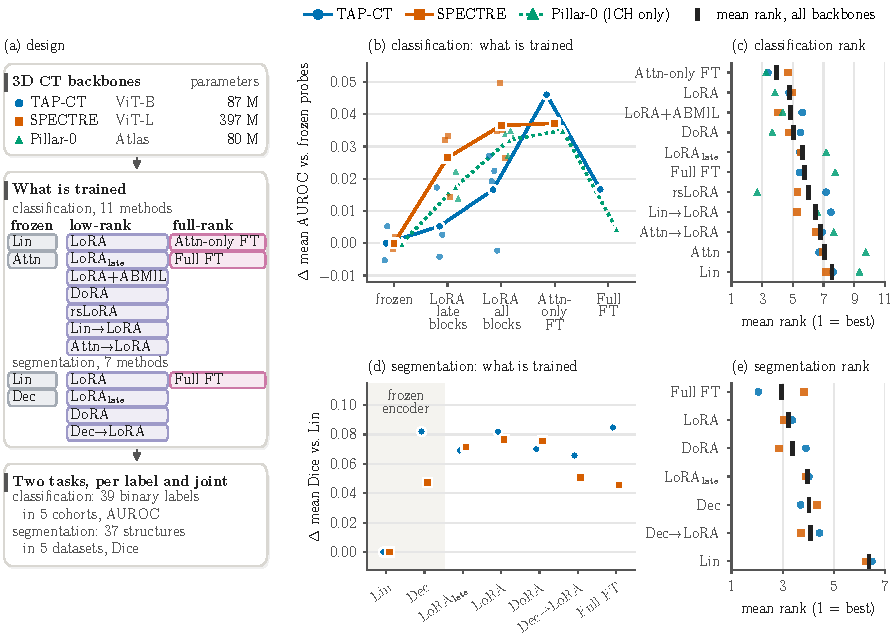
\includegraphics[width=\textwidth]{figures/fig_overview.pdf}
\vspace{-8pt}
\caption{Overview of the study. (a) Backbones, adaptation methods grouped by what they train, and tasks; Lin and Attn denote the linear and attentive probes and Dec the multi-depth decoder, all on the frozen encoder, and FT fine-tuning (Section~\ref{sec:ladder}). (b) Change in pooled held-out AUROC relative to the mean of each backbone's two frozen probes, where small markers denote methods (late blocks: LoRA$_{\text{late}}$ and the two-stage methods; all blocks: LoRA, LoRA+ABMIL, DoRA and rsLoRA) and lines group means. (c) Mean classification rank per backbone (markers) and pooled over backbones (bars). (d) Mean held-out Dice per segmentation method, computed on each backbone's own grid, where shading marks a frozen encoder. (e) Mean segmentation rank, as in (c). SPECTRE Full FT, which did not train, is excluded from (b) and (c); ranks are defined in Appendix~\ref{app:stats}.}
\label{fig:overview}
\end{figure}

A cohort collected for trauma or hemorrhage carries several findings per scan, and a segmentation dataset delineates several organs or lesions. Several pretrained 3D CT encoders are now public, among them TAP-CT \citep{veenboer2025tapct}, SPECTRE \citep{claessens2025spectre}, Pillar-0 \citep{agrawal2025pillar0}, CT-FM \citep{pai2025ctfm}, Merlin \citep{blankemeier2026merlin}, CT-CLIP \citep{hamamci2026ctrate} and FM-HCT \citep{zhu2025fmct}. Their evaluations mostly rank frozen representations with a linear, attentive or nearest-neighbor head \citep{veenboer2025tapct,claessens2025spectre}, and only some report end-to-end fine-tuning alongside \citep{pai2025ctfm,zhu2025fmct}. For natural images, comparisons on the same pretrained models showed that a frozen evaluation can be misleading. The linear-probe and fine-tuning accuracies of masked autoencoders were largely uncorrelated, and tuning a single transformer block raised ImageNet accuracy from 73.5\% to 81.0\% \citep{he2022mae}. Similarly, prompt tuning with under 1\% of the parameters outperformed full fine-tuning on 20 of 24 tasks \citep{jia2022vpt}, and full fine-tuning outperformed linear probing in distribution but not under distribution shift \citep{kumar2022lpft}. For 3D medical images such as CT, comparisons of this kind are few. Nonetheless, a group that adapts an encoder to a multi-label cohort or a multi-structure dataset, often with a few hundred to a few thousand labeled scans, has to decide whether to keep the encoder frozen, adapt it with low-rank adaptation (LoRA; \citealp{hu2022lora}) or fine-tune part or all of it, whether to train one model per label or one model for all labels of the dataset, and, for segmentation, which head turns the encoder tokens into a voxel map. A frozen probe answers none of these questions.

In medical imaging, the evidence for these choices comes mostly from 2D backbones and single tasks. On 2D medical classification, LoRA matches or surpasses full fine-tuning \citep{dutt2024peft,zhu2024melo}, and probing and fine-tuning of DINOv2 \citep{oquab2023dinov2} have been compared on radiology tasks \citep{baharoon2023dinov2med}. For 3D classification, \citet{liu2025anymc3d} found that frozen probing understates 2D and 3D foundation models, and that on the spleen-injury label of RSNA23 trauma, one of our labels, full fine-tuning of a convolutional and a Swin 3D model outperformed LoRA. Otherwise, parameter-efficient adaptation of 3D medical encoders has mostly been studied for segmentation, with adapters that lift the 2D Segment Anything model \citep{kirillov2023sam} to volumes \citep{gong20243dsamadapter,chen2024masam,wu2025medsa}, prompt tuning of a 3D U-Net \citep{fischer2024prompttuning}, and LoRA, adapters and full fine-tuning in few-shot transfer \citep{silvarodriguez2025fseft,ly2026seapeft}. For a 3D CT vision--language model, full and parameter-efficient fine-tuning performed similarly on one classification task \citep{kartika2026hcc}. However, each of these studies uses one backbone and one task, and none includes LoRA variants \citep{liu2024dora,kalajdzievski2023rslora}, probing before fine-tuning \citep{kumar2022lpft} or attention-only fine-tuning \citep{touvron2022three}. Joint training on many labels can help \citep{kim2023ctan} or hurt through conflicting gradients \citep{yu2020pcgrad,zhao2023mtlreview}. Yet joint and per-task adaptation of a 3D encoder have not been compared on the same labels \citep{veenboer2025tapct,liu2025anymc3d}. Our work aims to fill this gap.

To that end, we compared adaptation methods on five multi-label classification cohorts and five multi-structure segmentation datasets, under one protocol and on three encoders: two plain vision transformers (TAP-CT, SPECTRE) and the multi-scale transformer of Pillar-0 with its convolutional stem (Figures~\ref{fig:overview} and~\ref{fig:pipeline}). Classification was evaluated on all three encoders, with Pillar-0 on the head-CT cohort only and SPECTRE on the other four cohorts, and segmentation on TAP-CT and SPECTRE; every method was trained both per task and jointly. Our contributions can be summarized as follows:
\begin{itemize}\setlength{\itemsep}{1pt}
  \item We present a controlled comparison of \numClsMethodsN{} classification and \numSegMethodsN{} segmentation adaptation methods, ranging from frozen probes to low-rank adapters and full fine-tuning, on three 3D CT encoders from two architectural families, each trained per task and jointly (\numRunsMainN{} runs, plus \numRunsRevisionAllN{} repeats and controls).
  \item We find that, in classification, adapting the encoder's attention weights with LoRA outperforms both frozen probes on every encoder, whereas in segmentation a multi-depth decoder on the frozen encoder accounts for most of the gain, with LoRA beneath it changing Dice little on average.
  \item We find that one joint model per dataset performs on par with per-label models on average in classification but loses Dice in segmentation at our training budgets.
  \item We condense these findings into practical guidelines (Section~\ref{sec:guide}) and release our code, data splits and per-case predictions (\url{https://github.com/georgeyiasemis/beyond_frozen_encoders}).
\end{itemize}
